% This is LLNCS.DOC the documentation file of
% the LaTeX2e class from Springer-Verlag
% for Lecture Notes in Computer Science, version 2.4
\documentclass{llncs}
\usepackage{llncsdoc}
\usepackage[hyphens]{url}
\usepackage[pdftex]{graphicx}     
\usepackage{float}
\usepackage{tablefootnote}
\usepackage{hyperref}

\hyphenation{block-chain}
\hyphenation{block-chains}
\hyphenation{Block-chain}
\hyphenation{Block-chains}

	%%%%%%%%%%%%%%%%%%%%%%%
	%% Added to enable numbering for subsubsections, otherwise they would look like paragraphs which is ugly
	%%%%%%%%%%%%%%%%%%%%%%%
	
	\makeatletter
	\renewcommand\subsubsection{\@startsection{subsubsection}{3}{\z@}%
		{-18\p@ \@plus -4\p@ \@minus -4\p@}%
		{0.5em \@plus 0.22em \@minus 0.1em}%
		{\normalfont\normalsize\bfseries\boldmath}}
	\makeatother
	\setcounter{secnumdepth}{3}

%
\begin{document}


	{
	%
	\title{title\\ - \\ \small Research Paper - Version 0.0\\\small \today}
	
	\author{Benjamin Leiding \and William V. Vorobev}
	
	\institute{ 
		%Chorus Mobility a  Proof-of-Stake Inc. Project\\
		Chorus Mobility\\
		Email: hello@chorus.mobi\\
		%Website: chorus.technology	
	}
	
	\maketitle

	%% ----------------------------------------------------------------
	%% ----------------------------------------------------------------

	\begin{abstract}

		% A good abstract:
		%1.) What is the paper about?
		%2.) What is the SoA?
		%3.) What is the detected gap?
		%4.) What are the main questions to be answered pertaining to the gap?
		%5.) Why is the solution good/better than other solutions?

		The next generation of tightly interconnected vehicles offers a variety of new technologies as well as business opportunities. Vehicles form so-called vehicular ad hoc networks (VANETs). Sophisticated systems of interconnected cars in the context of VANETs assume a full coverage of 5G networks to unfold their full potential. However, nowadays network infrastructure is neither 5G-ready nor does it provide reliable and full coverage of all areas that might be relevant for VANET-based networks. Hence, the conventional mode of operations of all nodes being connected to one blockchain at all times is not feasible. In addition, traditional blockchains also require every node to process each transaction and smart contract commands which are highly inefficient. Therefore, we present a solution based on so-called mobile ad hoc blockchains that enable groups of nodes involved in any kind of collaboration to effectively form temporary networks and coordinate themselves. 

		Another critical requirement of VANETs and interconnected vehicles is security. The safety of network participants does not only depend on the vehicle's hardware, but also on the correctness of the software that controls the interaction and transaction within the network. Formal verification is a common way to address the issue proving the correctness of software. The self-amending blockchain Tezos supports Turing-complete smart contracts and also offers built-in formal verification of their programming languages, thereby fostering the security of our solution.

		This whitepaper fills the gap by introducing Vehicular Ad Hoc Tezos Blockchains based on mobile ad hoc blockchains that allow groups of nodes to be temporarily disconnected from the overall network but still being able to enact and transact on a local network level for the duration of their interaction. We present the advantages of the system, outline the requirements and goals, as well as the architecture of the system.



	\end{abstract}
	
	
	\keywords{VANET, Formal Verification, Tezos, Mobile Ad Hoc Blockchains, Blockchain, Smart Contracts, Interoperability, Vehicle Networks, V2X}

	%% ----------------------------------------------------------------
	%% ----------------------------------------------------------------
	
	\section{Introduction}
		\label{s:introduction}

		Despite steadily growing public transport networks and systems, especially in most first world countries, cars are still the default standard for urban transportation. In the US, ``about 86 percent of all workers commuted to work by private vehicle, either driving alone or carpooling" \cite{mckenzie2015drives}, even though in recent years the numbers remained relatively stable after decades of consistent increase. Similar applies to other industrial countries \cite{netherlandsPublicTransport}\cite{zealand2006car} though the overall percentage of vehicle commuters in Europe is lower than in the US \cite{commuteUSvsEurope}. While it was normal for the last few decades to own a vehicle and commute on a day-by-day basis, the future will be radically different due to the progressing evolution of self-driving cars and autonomous vehicles. The car-sharing economy that developed in recent years in combination with autonomous cars results in a so called \textit{passenger economy} \cite{intelPassengerEconomy}. Users no longer own cars, instead just hop on an autonomous car, pick a destination and get delivered without any human interaction. An Intel report estimates the size of this economy to be around US\$ seven trillion in 2050 \cite{intelPassengerEconomy}.

		\textbf{missing sources here - fix that}
		A key technology for the next generation of tightly interconnected vehicles are so-called vehicular ad-hoc networks (VANETs). Vehicles form VANETs enable vehicle-to-vehicle (V2V), vehicle-to-infrastructure (V2I), vehicle-to-human (V2H), or in general vehicle-to-everything (V2X) communication and interaction. In our previous research paper, we presented a blockchain-based system that enables a manufacturer agnostic platform solution that allows VANET participants to enact and transact any kind of services and goods. Sophisticated networks of interconnected cars require full coverage of 5G networks to unfold their full potential. However, nowadays network infrastructure is neither 5G-ready nor does it provide reliable and full coverage of all areas that might be relevant for VANET-based networks. Hence, the conventional mode of operations of all nodes being connected to one blockchain at all times is not feasible. In addition, traditional blockchains such as Bitcoin \cite{nakamoto_bitcoin:2008} and Ethereum \cite{wood2014ethereum} also require every node to process each transaction and smart contract commands which are highly inefficient. Therefore, we present a solution based on so-called mobile ad hoc blockchains that enable groups of nodes involved in any kind of collaboration to effectively form temporary networks and coordinate themselves. They only connect to nodes they need to be connected to, depending on the context, for the duration of their interaction.
		
		Another critical requirement of VANETs and interconnected vehicles is security. The safety of network participants does not only depend on the vehicle's hardware, but also on the correctness of the software that controls the interaction and transaction within the network. Formal verification is a common way to address the issue proving the correctness of software with respect to a certain formal specification or property using formal methods of mathematics. The self-amending blockchain platform Tezos \cite{tezosWhitepaper} does not only support Turing complete smart contracts, it also offers built-in formal verification of their smart contract programming languages, thereby fostering the security of our solution.
		\textbf{ADD some FV stuff + sources here}


%%%%%%%%%%%%%%%%%%%%%%%%%%%%%%%%%%%%%%%%%%%%%%%%%%%%%%%%%%%%%%%%%%%%%%

%		RQ: How to ?
%		RQ-1: What is the corresponding architecture of the Vehicular Ad Hoc Tezos Blockchain?
%		RQ-2: What are the detailed network and communication processes?
%		RQ-3: What kind of use cases and application scenarios exist?


%%%%%%%%%%%%%%%%%%%%%%%%%%%%%%%%%%%%%%%%%%%%%%%%%%%%%%%%%%%%%%%%%%%%%%
		
		This work fills the gap by introducing Tezos-based platform solution, thereby answering the question of how to enable vehicular ad hoc blockchains that allow groups of nodes to be temporarily disconnected from the overall network but still being able to enact and transact on a local network level for the duration of their interaction? In order to answer this question with a separation of concerns, we pose the following sub-questions: What is the corresponding architecture of the Vehicular Ad Hoc Tezos Blockchain? What are the detailed network and communication processes? What kind of use cases and application scenarios exist?
		
		The remainder of this paper is structured as follows: Section~\ref{s:section-2} introduces supplementary literature and related work. Section~\ref{s:section-3} outlines the system architecture our solution. Afterwards, Section~\ref{s:section-4} expands on the network communication processes, followed by Section~\ref{s:section-5} that introduces example use cases and application scenarios. Finally, Section~\ref{s:section-6} concludes this work and provides an outlook on future work.


	%% ----------------------------------------------------------------
	%% ----------------------------------------------------------------

	\section{Technical Background and Supplementary Literature}	
		\label{s:section-2}
		
		The following section provides background information and describes related works regarding previous ideas and concepts that focus on a blockchain-based VANET platforms. First, Section~\ref{ss:blockchain-intro} introduces the general concepts of blockchain technology, terms and frameworks. Afterwards, Section~\ref{ss:vanets} and Section~\ref{ss:formal-verification} focus on the fundamentals of vehicular ad-hoc networks as well as formal verification. Finally, Section~\ref{ss:related-work} introduces related work. 
					
		%% ----------------------------------------------------------------
		%% ----------------------------------------------------------------	
		
		\subsection{Blockchain Technology}
			\label{ss:blockchain-intro}
			
			As the name suggests, a blockchain consists of a chronologically ordered chain of blocks. Every block consists of a certain number of validated transactions and each of those block links to its predecessor by a hash reference. As a result, changing the content of one block also changes all succeeding blocks and hence breaks the chain. All blocks are stored on and verified by all participating nodes. While the initial Bitcoin blockchain only supported a very limited set of scripting instructions, the next generation of blockchain platforms, e.g., Ethereum \cite{wood2014ethereum}, Qtum \cite{qtumWhitepaper}, or Tezos \cite{tezosWhitepaper}, provide Turing-complete programming languages on the protocol-layer level in order to enable smart contract capabilities. Smart contracts are ``orchestration- and choreography protocols that facilitate, verify and enact with computing means a negotiated agreement between consenting parties" \cite{qtumWhitepaper}. Hence, the entities participating in the enactment of a smart contract establish binding agreements and deploy applications using such smart contracts in order to provide blockchain-based applications. Those application are as versatile as smart contracts itself and enable services including the finance sector \cite{nguyen2016blockchain}\cite{saltWhitepaper}, academic and business authentication and identity solutions \cite{leidingUnchained}\cite{CivicWhitepaper}\cite{AuthcoinLeiding2016MCIS}\cite{mccorry2015authenticated}\cite{SelfkeyWhitepaper}, reputation systems \cite{SemadaWhitepaper} as well as platforms for Internet-of-Things (IoT) applications \cite{christidis2016blockchains}\cite{ouaddah2017towards}. 	
			
			The blockchain concept is particularly interesting for the V2X economy for three reasons. First, it removes the need for trusted third parties and instead enables trust-less transaction enactment. Second, transactions that were agreed up on cannot be changed later on since the underlying blockchain is tamperproof. Third, no human interaction is required for any kind of transaction between vehicles or machines in general.


		%% ----------------------------------------------------------------
		%% ----------------------------------------------------------------	
		
		\subsection{Vehicular Ad-Hoc Networks - VANETs}
			\label{ss:vanets}

			Communication between vehicles, road infrastructure and Internet-based services is a key enabler for the upcoming generation of vehicles. So called vehicular ad-hoc networks provide an abstract concept that models the different components that are required for V2V, V2I, or V2X communication. Figure \ref{fig:vanets} illustrates the main components of VANETs: Vehicles, on-board-units (OBUs), application-units (AUs) and road-side-units (RSUs).\\
			RSUs are placed  along the road side or in dedicated locations such as at crossroads. Typically, RSUs provide short range communication based on IEEE 802.11p radio technology but can also be equipped with other network devices in order to provide communication within the infrastructural network \cite{al2014comprehensive}. OBUs are mounted onto a vehicle and used for data exchange. To do so, short range wireless- or radio communication is used to exchange these information \cite{baldessari2007car}. Closely linked to the OBU is the AU, they might even reside in the same physical unit or as a mobile until that is regularly removed from the vehicle (e.g smartphones). The AU provides an execution environment for applications that utilize the OBU's communication capabilities \cite{al2014comprehensive}\cite{baldessari2007car}.\\	
			\begin{figure}[ht]
				\centering
				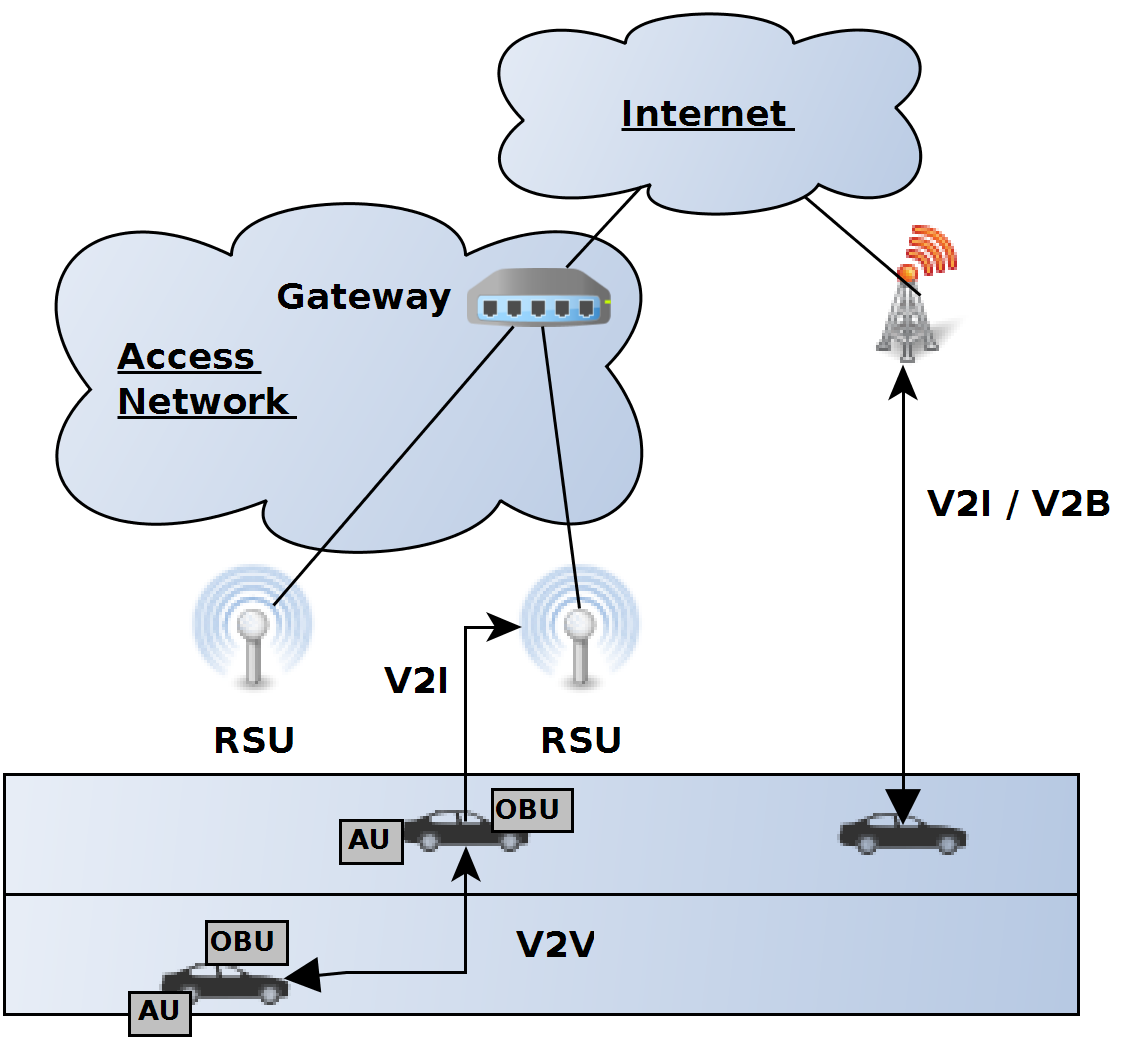
\includegraphics[scale=0.2]{Figures/Vanets.png}
				\caption{General VANET architecture (Based on \protect\cite{baldessari2007car} and \cite{leiding2016self})}
				\label{fig:vanets}
			\end{figure}			
			Communication in VANETs occurs either inside a vehicle between AUs and OBU, wirelessly between different vehicles (V2V), vehicles and infrastructure (V2I) or vehicles and the infrastructure via broadband (V2B) \cite{faezipour2012progress}. For authentication purposes, each network participant is equipped with a unique public/private key pair that resides in a tamper-proof-device (TPD). In blockchain terms, the TPD is similar to an external hardware wallet.

		%% ----------------------------------------------------------------
		%% ----------------------------------------------------------------	
		
		\subsection{Formal Verification}
			\label{ss:formal-verification}
			
			basic introduction with motivation, advantages and disadvantages
			A380 example?
			
			
			connect formal verification and blockchain
			tezos
			cardano
			others?
		%% ----------------------------------------------------------------
		%% ----------------------------------------------------------------	
		
		\subsection{Related Work}
			\label{ss:related-work}

			
			
		%% ----------------------------------------------------------------
		%% ----------------------------------------------------------------	
		

	%% ----------------------------------------------------------------
	%% ----------------------------------------------------------------

	\section{System Design and Architecture}
		\label{s:section-3}
		
		%% ----------------------------------------------------------------
		%% ----------------------------------------------------------------	
		
		\subsection{System Architecture}
			\label{ss:architecture-overview}
		
		
		
		%% ----------------------------------------------------------------
		%% ----------------------------------------------------------------	

		\subsection{Identities}
			\label{ss:identities}
		
			involve Authcoin \cite{leiding2017securing}\cite{AuthcoinLeiding2016MCIS}\cite{leiding2017mapping}
		
		%% ----------------------------------------------------------------
		%% ----------------------------------------------------------------	

		\subsection{Blockchain Consensus in VANETs}
			\label{ss:consensus}
		
		
		
		%% ----------------------------------------------------------------
		%% ----------------------------------------------------------------	
				
	

	%% ----------------------------------------------------------------
	%% ----------------------------------------------------------------
	
	
	\section{Network and Communication}
		\label{s:section-4}	

		%% ----------------------------------------------------------------
		%% ----------------------------------------------------------------	
		
		\subsection{Inter-Blockchain Communication}
			\label{ss:inter-blockchain-communication}
			
		%% ----------------------------------------------------------------
		%% ----------------------------------------------------------------	

		\subsection{Network Communication}
			\label{ss:network-communication}
		
			+5g
		%% ----------------------------------------------------------------
		%% ----------------------------------------------------------------	

		\subsection{Hubs}
			\label{ss:blockchain-hubs}
		
		%% ----------------------------------------------------------------
		%% ----------------------------------------------------------------	


	

	%% ----------------------------------------------------------------
	%% ----------------------------------------------------------------
	
	\section{Use Cases and Application Scenarios}
		\label{s:section-5}	
	
	
	
	%% ----------------------------------------------------------------
	%% ----------------------------------------------------------------

	\section{Conclusion and Future Work}
		\label{s:section-6}	

		This whitepaper presents

%		This whitepaper presents the Chorus Mobility blockchain-based transaction and interaction layer that enables a V2X platform for goods and services. We outline and describe the technical foundations of this new economy, the longterm vision and benefits as well as the different use cases and scenarios of V2X transactions and interactions, e.g., vehicle-to-vehicle (V2V), vehicle-to-human (V2H), or vehicle-to-infrastructure (V2I).
%		
%		Based on the use cases and scenarios we identify the requirements and criteria that a blockchain-based V2X transaction and interaction layer protocol must satisfy. With respect to functional and non-functional requirements, Chorus aims to develop a blockchain- as well as manufacturer agnostic and interoperable V2X platform that enables interaction and transaction between participating entities and a plug-in interface for external applications.
%		Subsequently, we derive the service-oriented architecture of the system based on the identified requirements and goals. We present the system architecture using technology-agnostic UML-component and sequence diagrams that detail the system’s main components and communication interfaces. In order to ensure widespread adoption, special focus will be given in the future to the API design and library integration for car manufacturers.
%		
%		A core element of many of the Chorus use cases is smart contract-based negotiation and contract enactment between
%		entities that are the result of collaborating tasks and subprocesses. On an abstract level, most of the use cases presented in this paper follow a similar workflow on the smart-contract level. Hence, we decided to integrate an abstract smart contract negotiation lifecycle that we describe. The lifecycle is divided into the different stages (preparatory, negotiation, contract execution, rollback and contract expiry stage) that we explain in detail. Furthermore, we designed two auction algorithms for the V2X economy that allow to reach an efficient consensus on a certain price between buyer and seller. Our auction algorithms are based on the concept of so called Vickrey Auction, and we envisioned one algorithm for one-to-one interaction as well as a second workflow for scenarios with multiple buyers and sellers. Finally, we present the Chorus token value proposition and the surrounding token economy eco-system that fuels the V2X platform.
%		
%		Next, we present a Chorus prototype implementation. We demonstrate how our protocol can help mitigating traffic congestions and at the same time provides a mean to car insurance companies to incentivize their customers to practice good driving behavior. 	
%		
%		Future releases will focus on the longterm vision of Chorus Mobility and the development of the abstract transaction and interaction layer as well as the API and library integration. Besides that, we will also continue to focus on further research aspects of the upcoming V2X economy that will facilitate future developments of Chorus Mobility.


	%% ----------------------------------------------------------------
	%% ----------------------------------------------------------------
	
	\section{Notes}
		\label{s:section-7}	
	
		\begin{itemize}
			\item somehow get FOAM \cite{foamWhitepaper} into this?
		\end{itemize}

	%% ----------------------------------------------------------------
	%% ----------------------------------------------------------------


	\label{Bibliography}
	\bibliographystyle{splncs03}
	\bibliography{Bibliography}
	
	%% ----------------------------------------------------------------
	%% ----------------------------------------------------------------	



	%
\end{document}


